We validate the fit performance of the $2_m^+$ model in the same way as in the SM Higgs analysis~\cite{HWWMoriond2013} by 
doing toy MC experiments under different initial conditions.
Goal of the study is to determine the fit resolution and to check that it does not lead to 
biases in the signal strenght measurement. 
In this section we document the results on the most sensitive channels in the 0-Jet bin for the major systematic sources. 

We first test the fit performance without any input bias. 
Figure~\ref{fig:toyfit_statonly_0j} show the distributions of the relative fit biases 
for the signal and key background processes in the 0 jet bin. 
The signal is estimated with negligible bias ($\sim 1$\%) and the resolution is 31\% 
when toy are sampled with statistical variations only. 
On average we do not find biases on the main background processes either. 
We have also tested the fit performance including systematic effects, where the 
toy datasets are generated sampling over all the systematic nuisance parameters except the normalization 
uncertainties on the $WW$ as it is floated freely in the fit. 
Figure~\ref{fig:toyfit_0j} show the distributions of the relative fit biases 
for the signal and key background processes in this configuration.  
We find that including the systematic effects does not introduce additional bias on both 
signal and background yields. But it worsens the signal resolution by $\sim$30\% as expected.  


%%%%%%%%%%%%%%%%%%%%%%%%%%%%%% 
\begin{table}
\begin{center}
\begin{tabular}{c | c  | c c | c c | c c | c c | c c }
\hline
\hline
          &      & \multicolumn{2}{c|}{{\bf ggH}} & \multicolumn{2}{c|}{qqWW} & \multicolumn{2}{c|}{Top} & \multicolumn{2}{c}{WjetsM} & \multicolumn{2}{c}{WjetsE} \\ 
N$_{jets}$ & Test & bias & $\sigma$ & bias & $\sigma$ & bias & $\sigma$ & bias & $\sigma$ & bias & $\sigma$ \\
\hline
0 & default                             &  -1 & 31 &-0.5 & 3 &  2  & 11 & 0.1 & 15 &-0.3 & 10 \\
0 & sampling: stat.+syst.               &  -4 & 41 & 0.7 & 6 &  6  & 21 &  2  & 17 & -1  & 11 \\
\hline
0 & analysis: inflated Wjets error      &  -2 & 36 & -0.5 & 3 &  2  & 11 &  3        & 29 & -1   & 10 \\
0 & input: WjetsM {\bf +36\% bias}      &  16 & 31 & 0.3  & 3 & 0.1 & 11 & {\bf 15}  & 20 & 2    & 10 \\
0 & input: WjetsM {\bf -36\% bias}      & -15 & 28 & -1   & 3 & 3   & 11 & {\bf -12} & 12 & -4   & 9 \\
%0 & input: WjetsM from altern. shape    & -4  & 25 & -0.1 & 3 & 2   & 11 & 6         & 15 & -0.5 & 10 \\
\hline
0 & input: qqWW {\bf +10\% bias}        & 2 & 31 & {\bf 9}   & 3 & 1 & 11 & -0.1 & 16 & -1   & 10 \\
0 & input: qqWW {\bf -10\% bias}        & 2 & 29 & {\bf -10} & 3 & 1 & 11 & -1.5 & 15 & -0.8 & 10 \\
%0 & input: qqWW from altern. shape      & -2  & 27 & -0.1      & 3 & 2   & 12 & 6   & 15 & -2  & 10 \\
\hline
0 & input: Top {\bf +20\% bias}         & -1  & 30  & 1    & 3 & {\bf 12} & 12  & -2 & 14  & -1   & 10\\
0 & input: Top {\bf -20\% bias}         & 4   & 30  & -2   & 3 & {\bf -8} & 10  & 2  & 15  & -0.2 & 10\\
%0 & input: Top from altern. shape       & -2  & 27  & -0.6 & 3 & 5        & 11  & 8    & 16  & -1   & 9\\
%\hline
%\hline
%1 & default                             & -3  & 35 & 2   & 9  & -2  & 5 & -0.1 & 20 & -2 & 12 \\
%1 & sampling: stat.+syst.               & -6  & 48 & 3   & 16 & 0.4 & 6 & 0.6  & 25 & 0.7& 14 \\
%\hline
%1 & analysis: inflated Wjets error      &  -3 &  37 & 2  & 9 & -2   & 5  & 0.1      & 24  & -2  & 12 \\ 
%1 & input: WjetsM {\bf +36\% bias}      &  5  &  35 & 4  & 9 & -2   & 5  & {\bf 26} & 26  & 1   & 12 \\ 
%1 & input: WjetsM {\bf -36\% bias}      & -14 &  33 & 0.5& 9 & -1   & 5  & {\bf-20} & 15  & -5  & 11 \\ 
%1 & input: WjetsM from altern. shape    &  -3 &  35 & 1  & 8 & -0.3 & 5  & 17       & 21  & -1  & 12 \\
%\hline
%1 & input: qqWW {\bf +10\% bias}        & 4   & 37 & {\bf 12} & 9 & -2  & 5  & 0.3  & 19 & 1  & 11 \\
%1 & input: qqWW {\bf -10\% bias}        & -1  & 33 & {\bf -7} & 9 & -2  & 5  & 0.3  & 18 & -2 & 13 \\
%1 & input: qqWW from altern. shape      & -2  & 37 & 2        & 8 & -1  & 4  & 14   & 22 & -3 & 12 \\
%\hline
%1 & input: Top {\bf +5\% bias}          & -6   & 35  & 8   & 9 & {\bf -0.5} & 5 & -1 & 17 & -2 & 11 \\
%1 & input: Top {\bf -5\% bias}          & -2   & 35  & -2  & 9 & {\bf -3}   & 5 & 2  & 19 & -1 & 12 \\
%1 & input: Top from altern. shape       & -0.3 & 33  & 0.6 & 8 & 0.3        & 5 & 17 & 21 & -2 & 12 \\
\hline
\hline
\end{tabular}
\caption{Summary of results from toy experiments. Values of bias and $\sigma$ are \%.
In the Test column, ``default'' stands for: sampling is statistical only, input is nominal, analysis is nominal; 
in all other cases, the difference with respect to default is stated.}
\label{tab:toy_summary}
\end{center}
\end{table}



%%%%%%%%%%%%%%%%%%%%%%%%%%%%%%%%%%%%
\begin{figure}[!hbtp]
\centering
\subfigure[ggH]{
\centering
\label{subfig:ggh}
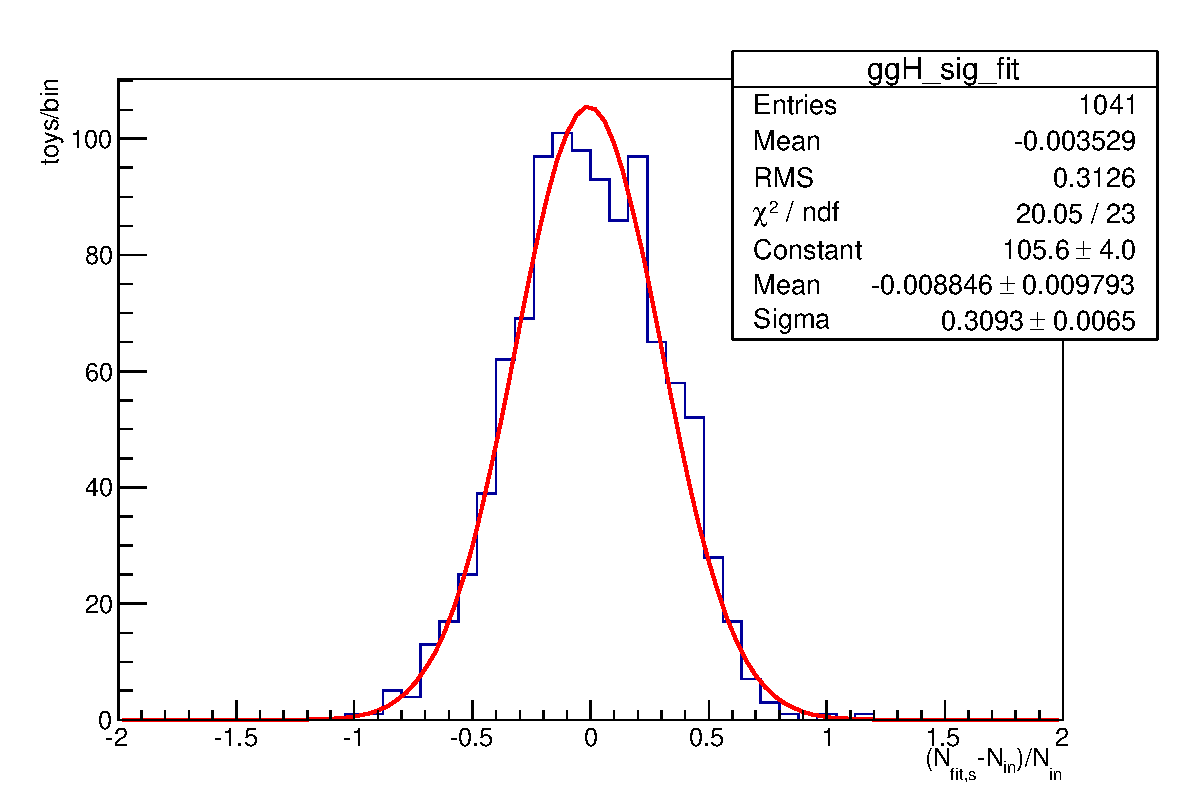
\includegraphics[width=.45\textwidth]{figures/norm_inj125_0j_125_sfit_ggH_xww_statonly.pdf}
}
\subfigure[qqWW]{
\centering
\label{subfig:qqww}
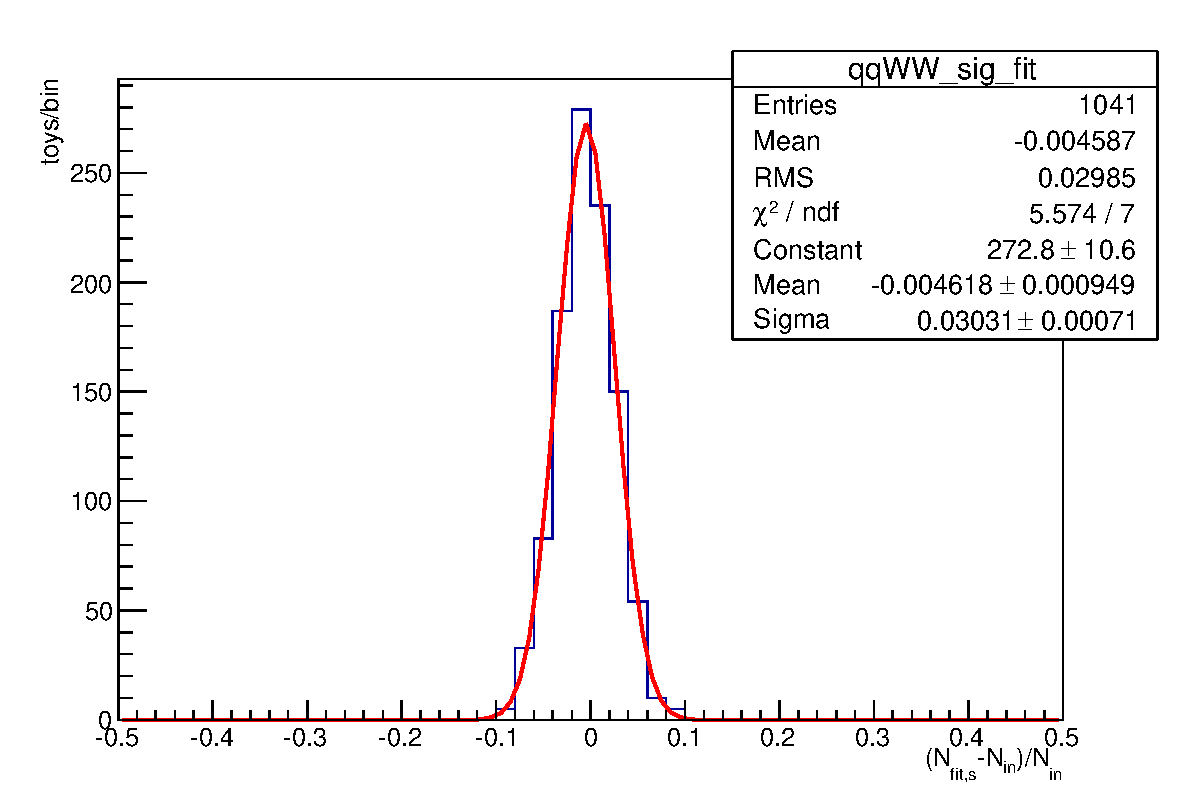
\includegraphics[width=.45\textwidth]{figures/norm_inj125_0j_125_sfit_qqWW_xww_statonly.pdf}
}\\
\subfigure[ggWW]{
\centering
\label{subfig:ggww}
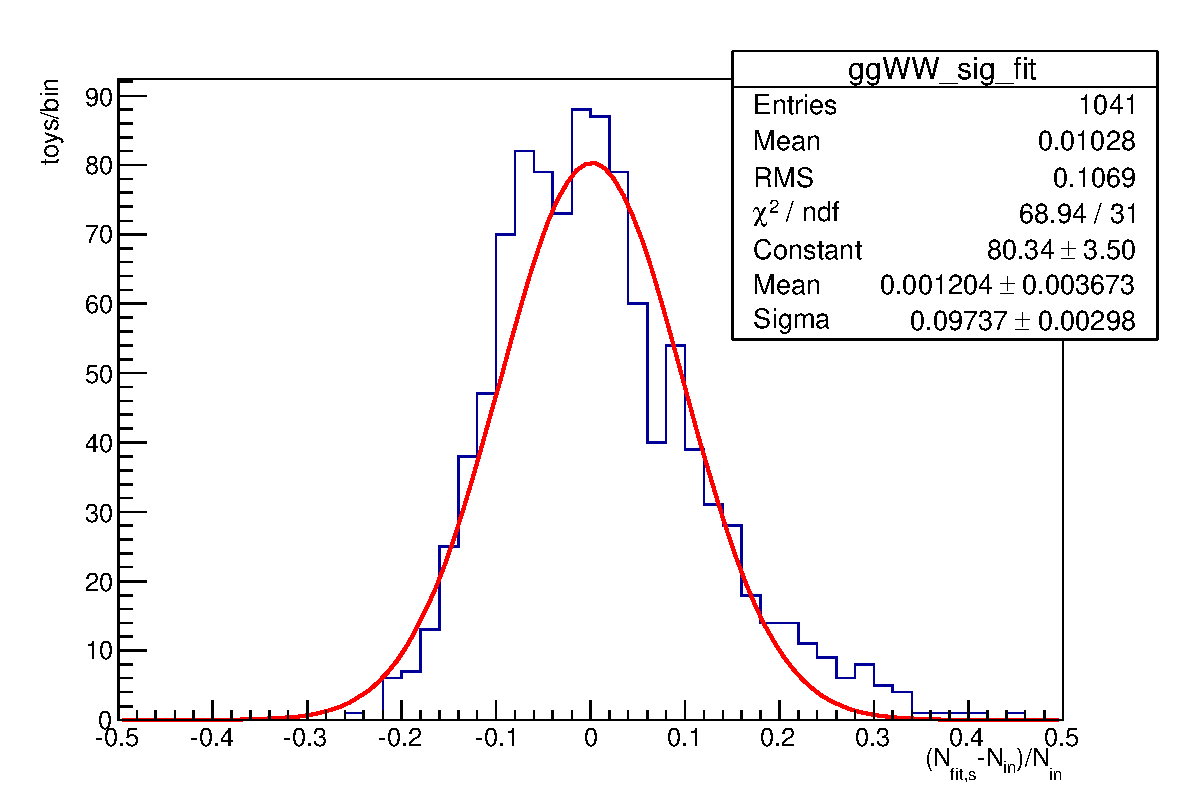
\includegraphics[width=.45\textwidth]{figures/norm_inj125_0j_125_sfit_ggWW_xww_statonly.pdf}
} 
\subfigure[Top]{
\centering
\label{subfig:top}
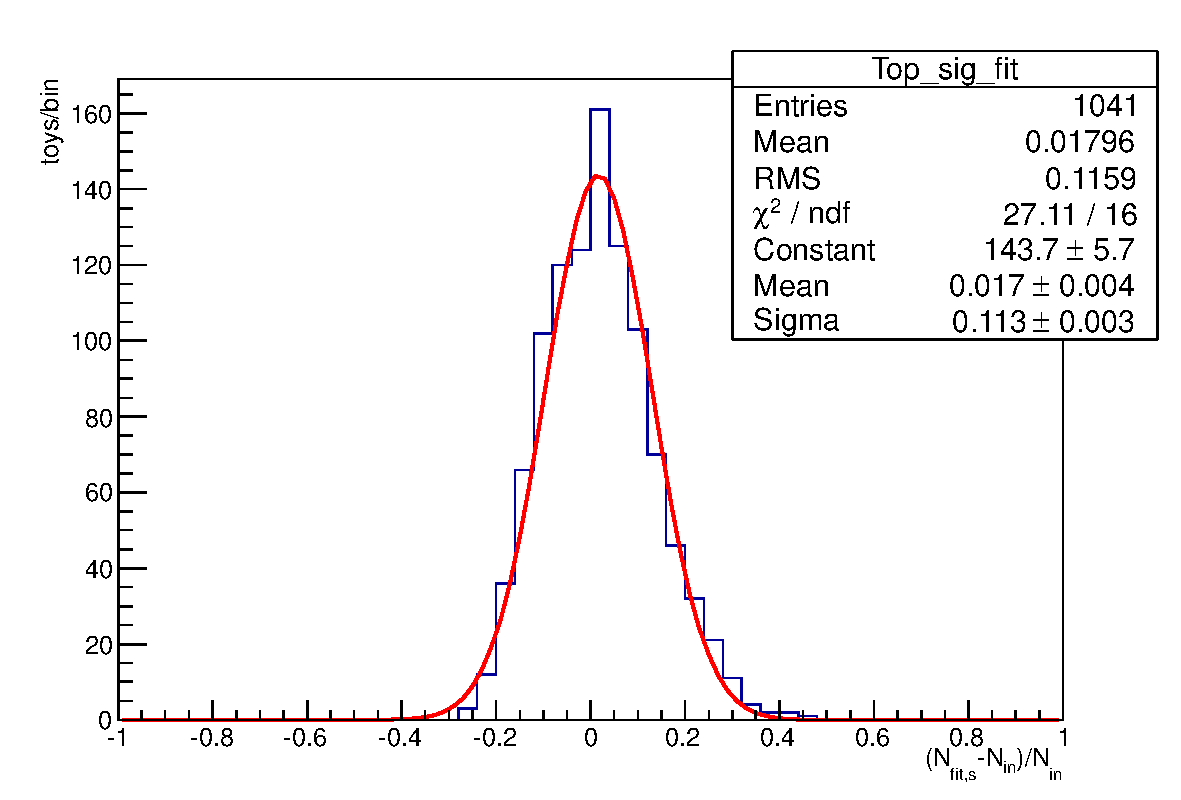
\includegraphics[width=.45\textwidth]{figures/norm_inj125_0j_125_sfit_Top_xww_statonly.pdf}
} \\
\subfigure[WjetsE]{
\centering
\label{subfig:wjetse}
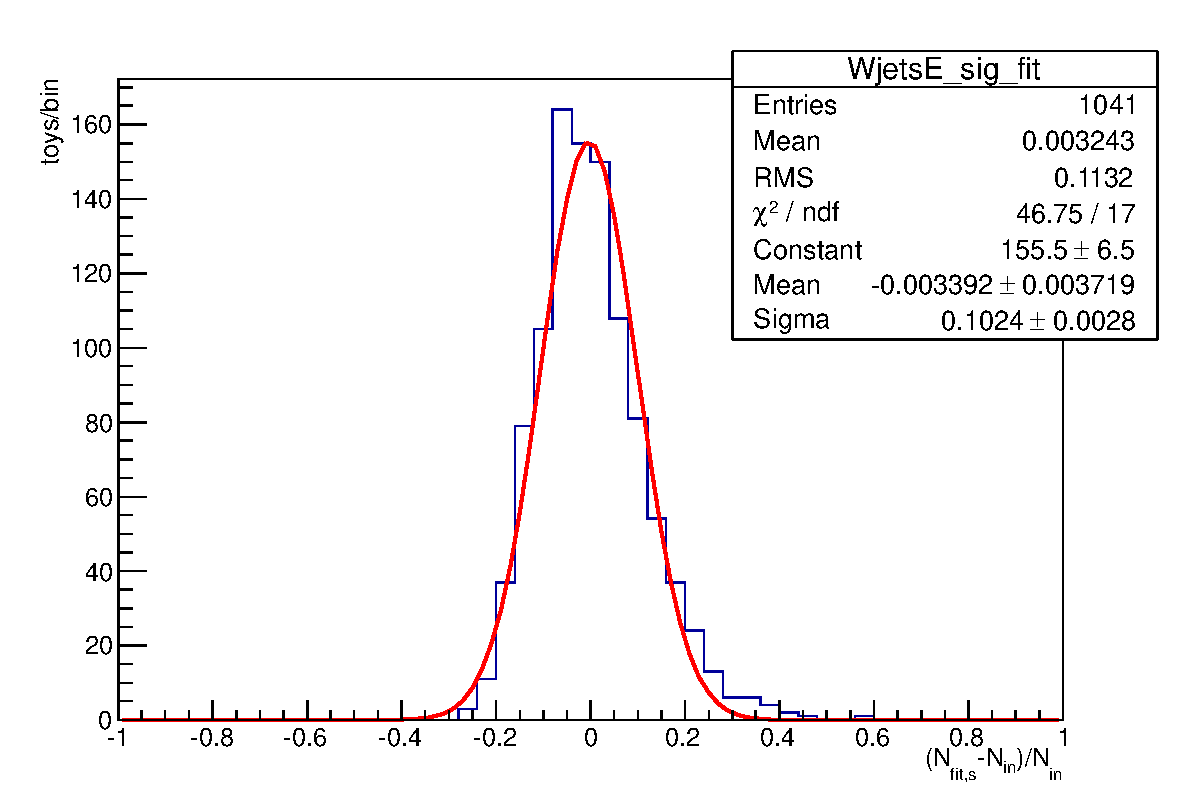
\includegraphics[width=.45\textwidth]{figures/norm_inj125_0j_125_sfit_WjetsE_xww_statonly.pdf}
} 
\subfigure[WjetsM]{
\centering
\label{subfig:wjetsm}
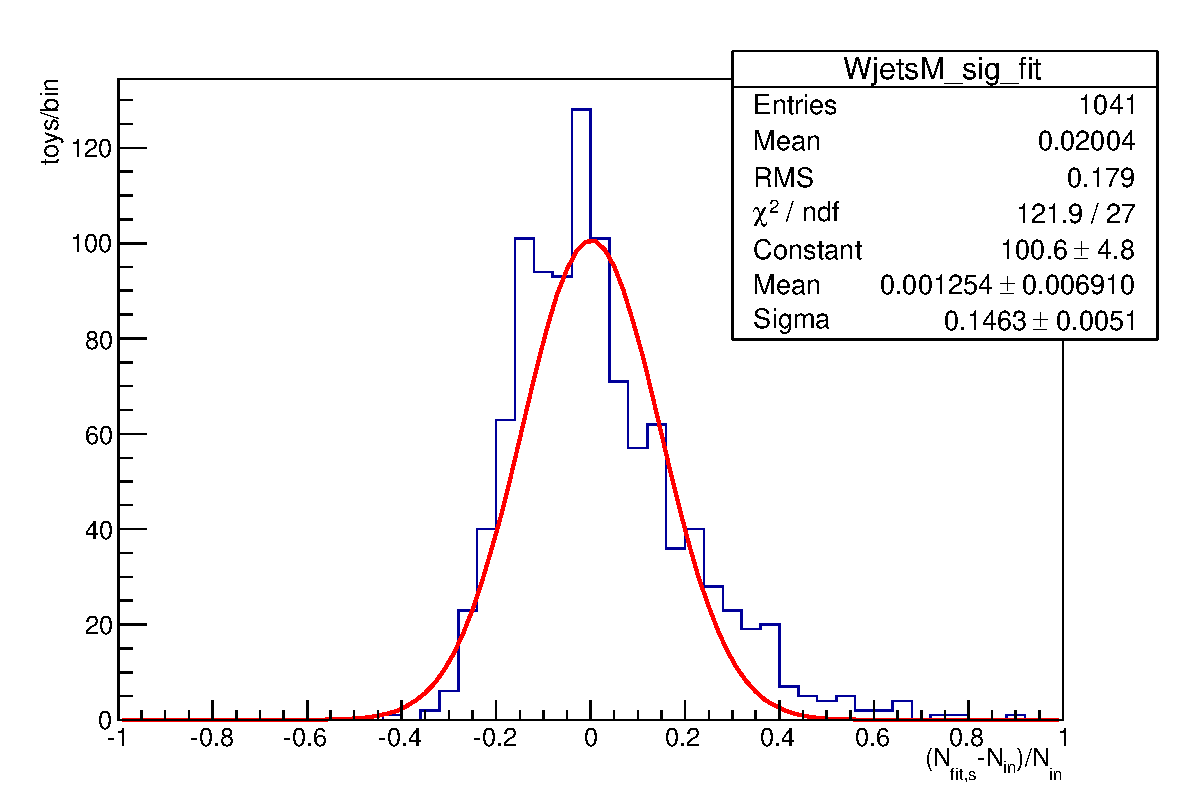
\includegraphics[width=.45\textwidth]{figures/norm_inj125_0j_125_sfit_WjetsM_xww_statonly.pdf}
} 
\subfigure[W$\gamma$]{
\centering
\label{subfig:wgamma}
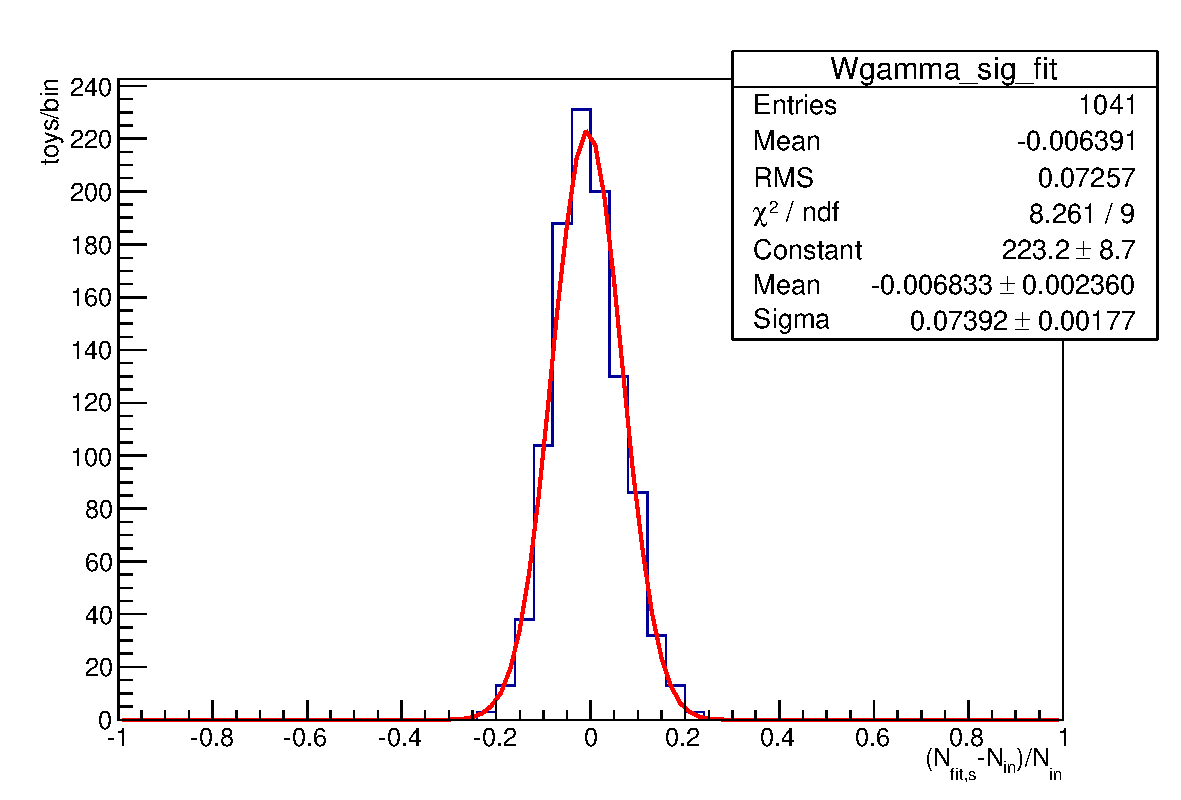
\includegraphics[width=.45\textwidth]{figures/norm_inj125_0j_125_sfit_Wgamma_xww_statonly.pdf}
} 
\subfigure[W$\gamma^*$]{
\centering
\label{subfig:wg3l}
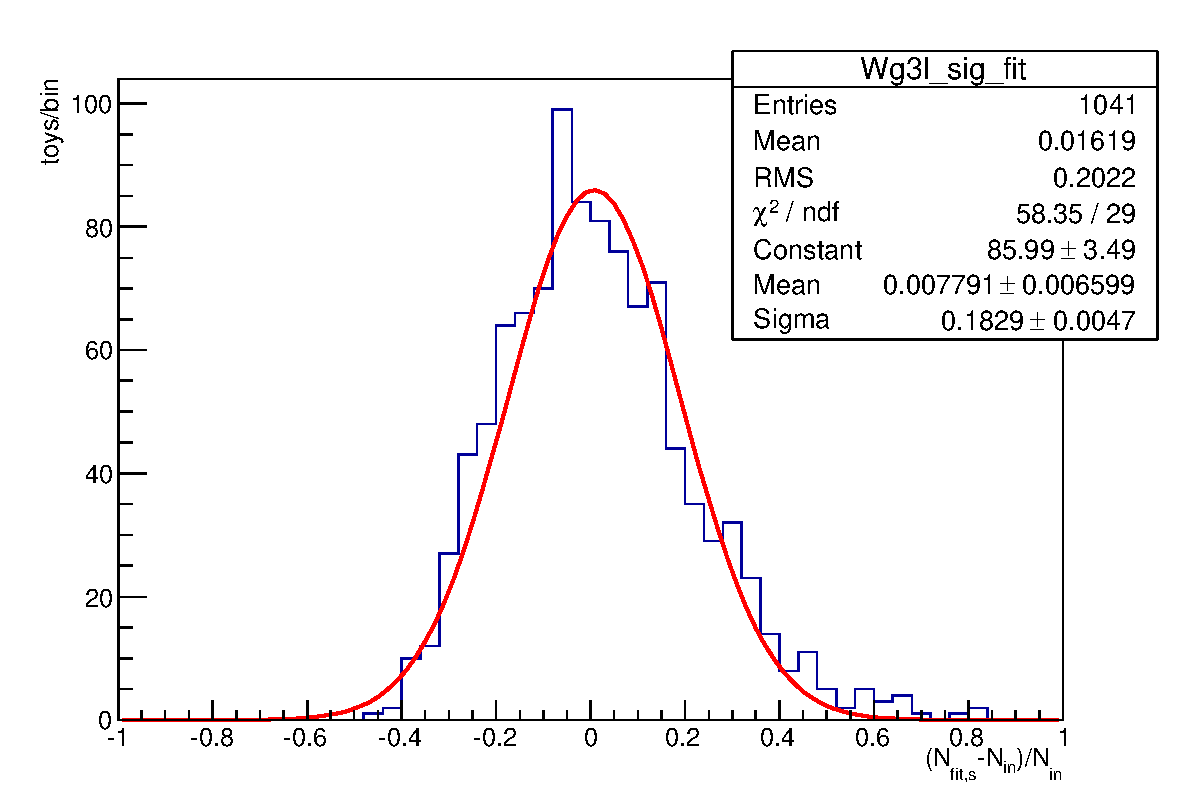
\includegraphics[width=.45\textwidth]{figures/norm_inj125_0j_125_sfit_Wg3l_xww_statonly.pdf}
} 

\caption{The relative fit bias $(N_{\text fit} - N_{\text in})/N_{\text in}$ distributions 
of the main signal and background processes in the toy MC based fit studies in the {\bf 0-Jet bin}. 
The toy datasets are generated sampling {\bf only statistics of the templates}. }
\label{fig:toyfit_statonly_0j}
\end{figure}
%%%%%%%%%%%%%%%%%%%%%%%%%%%%%%%%%%%%



%%%%%%%%%%%%%%%%%%%%%%%%%%%%%%%%%%%%
\begin{figure}[!hbtp]
\centering
\subfigure[ggH]{
\centering
\label{subfig:ggh}
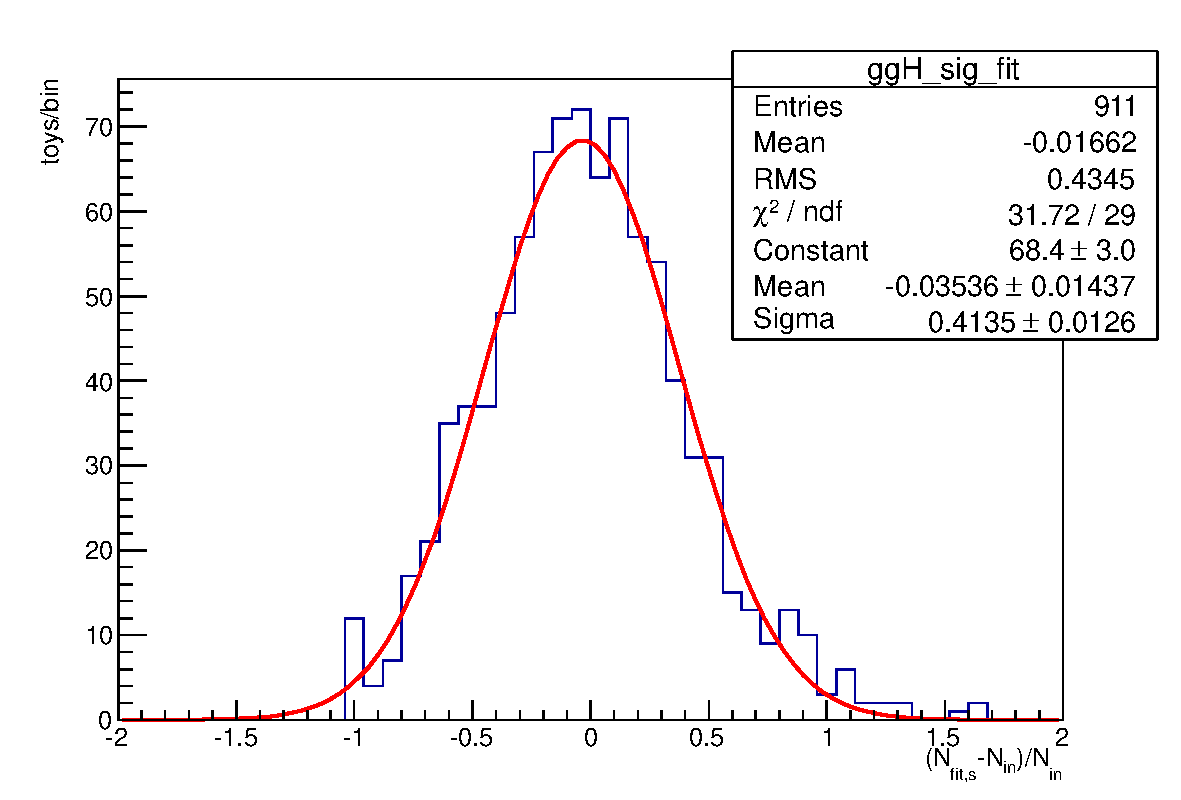
\includegraphics[width=.45\textwidth]{figures/norm_inj125_0j_125_sfit_ggH_xww.pdf}
}
\subfigure[qqWW]{
\centering
\label{subfig:qqww}
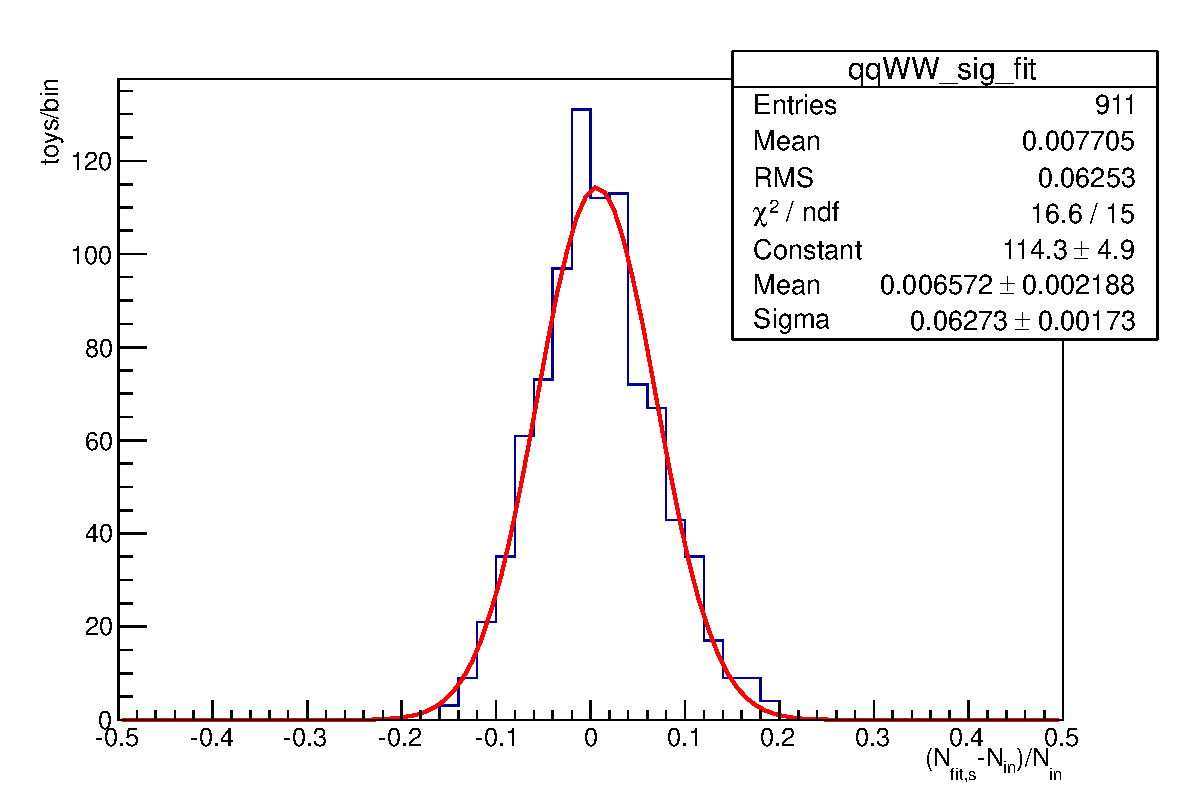
\includegraphics[width=.45\textwidth]{figures/norm_inj125_0j_125_sfit_qqWW_xww.pdf}
}\\
\subfigure[ggWW]{
\centering
\label{subfig:ggww}
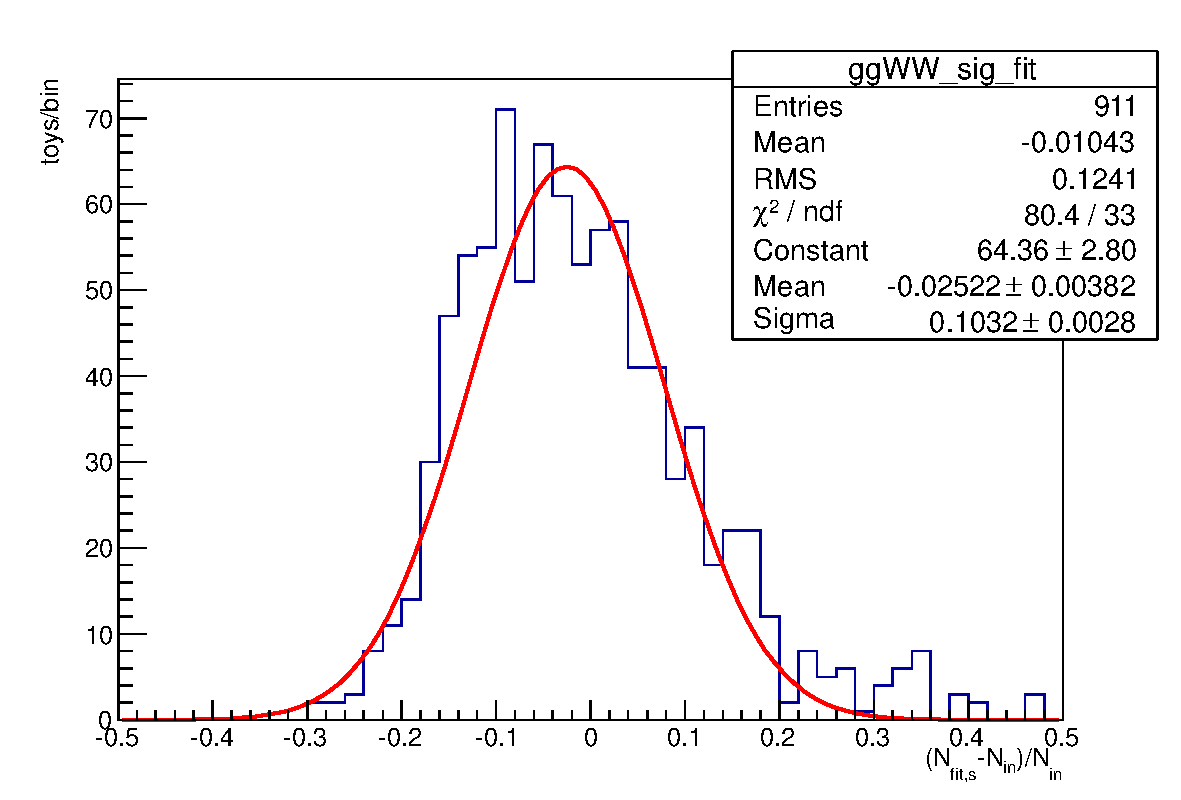
\includegraphics[width=.45\textwidth]{figures/norm_inj125_0j_125_sfit_ggWW_xww.pdf}
} 
\subfigure[Top]{
\centering
\label{subfig:top}
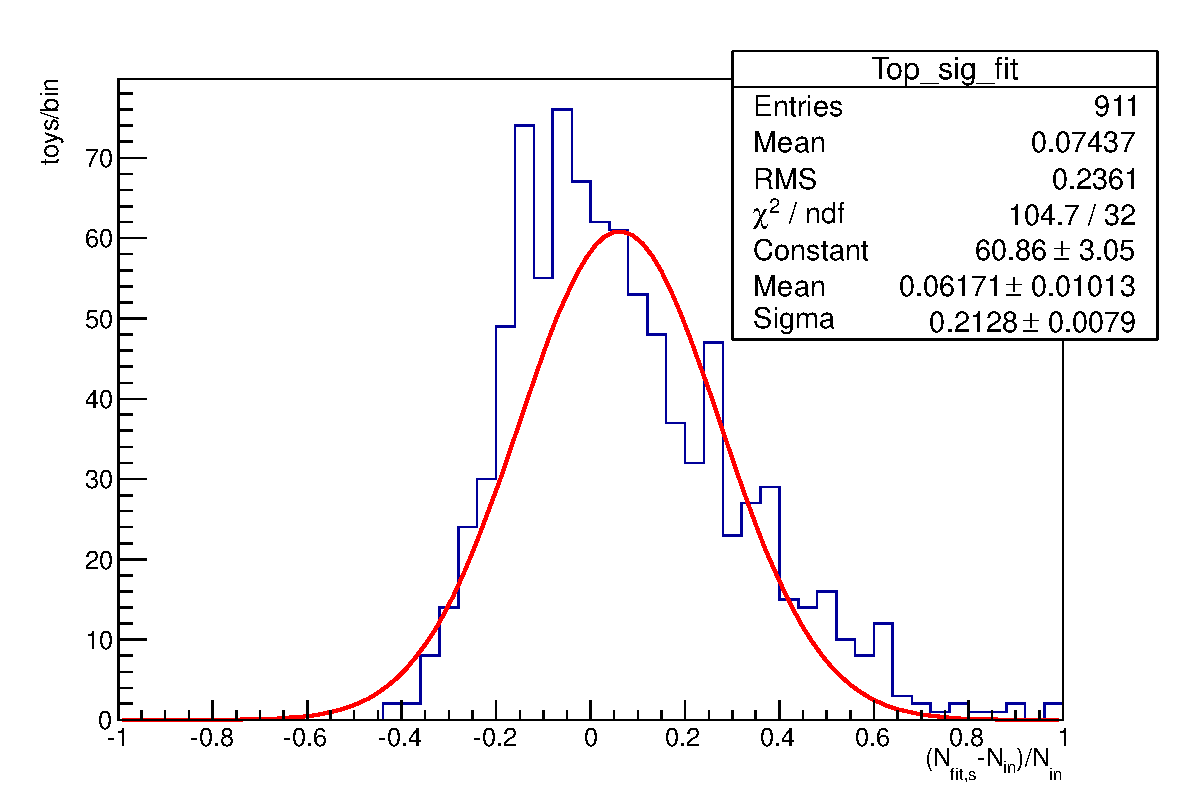
\includegraphics[width=.45\textwidth]{figures/norm_inj125_0j_125_sfit_Top_xww.pdf}
} \\
\subfigure[WjetsE]{
\centering
\label{subfig:wjetse}
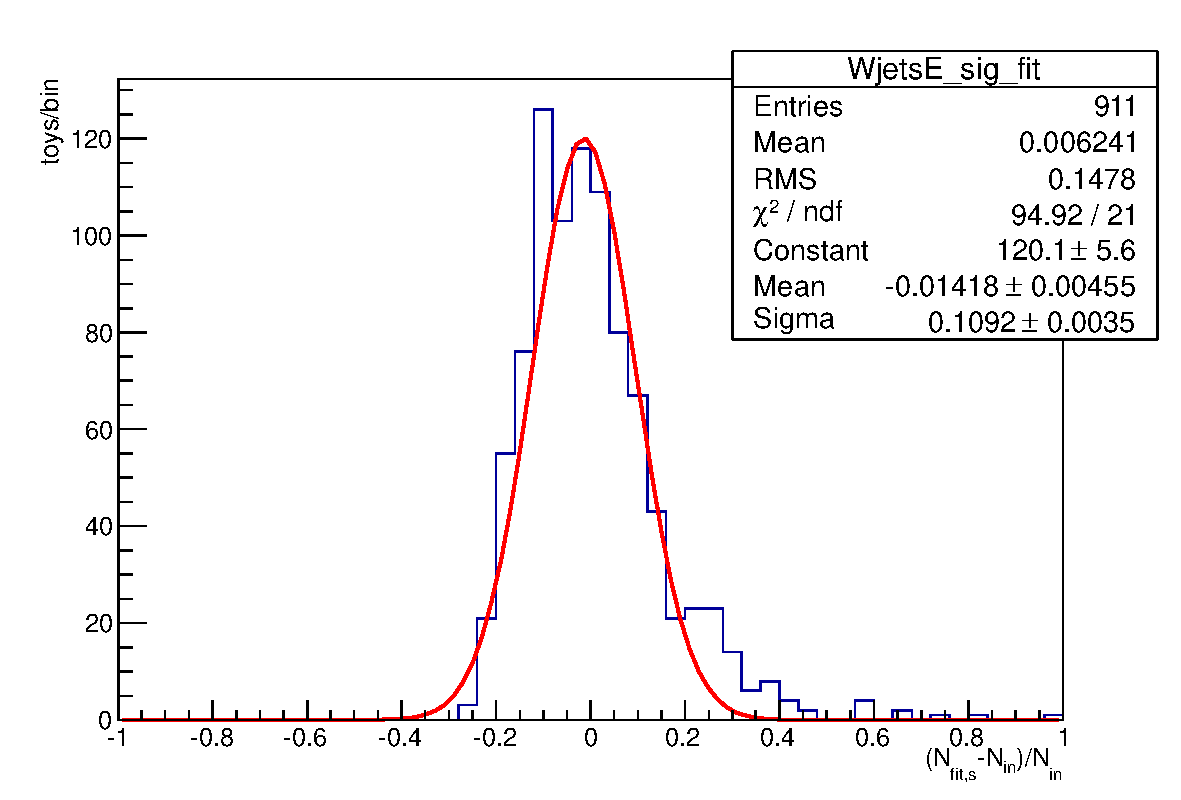
\includegraphics[width=.45\textwidth]{figures/norm_inj125_0j_125_sfit_WjetsE_xww.pdf}
} 
\subfigure[WjetsM]{
\centering
\label{subfig:wjetsm}
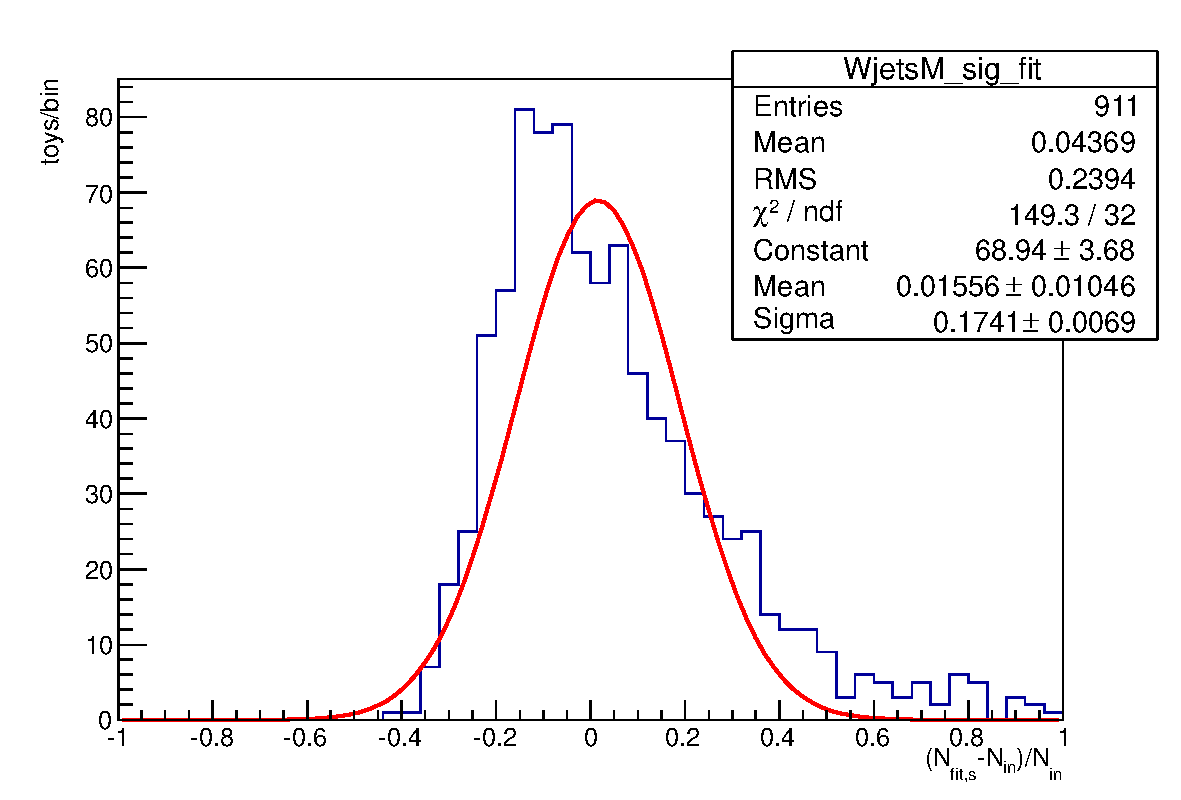
\includegraphics[width=.45\textwidth]{figures/norm_inj125_0j_125_sfit_WjetsM_xww.pdf}
} 
\subfigure[W$\gamma$]{
\centering
\label{subfig:wgamma}
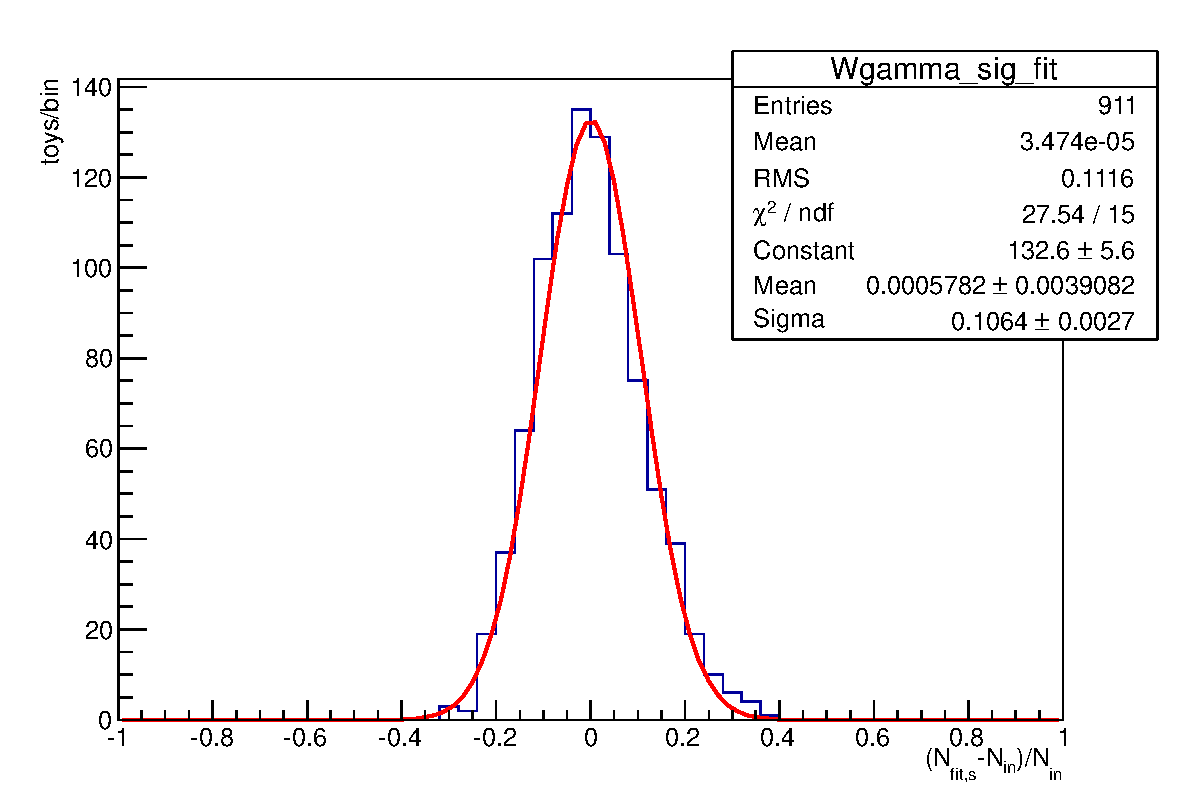
\includegraphics[width=.45\textwidth]{figures/norm_inj125_0j_125_sfit_Wgamma_xww.pdf}
} 
\subfigure[W$\gamma^*$]{
\centering
\label{subfig:wg3l}
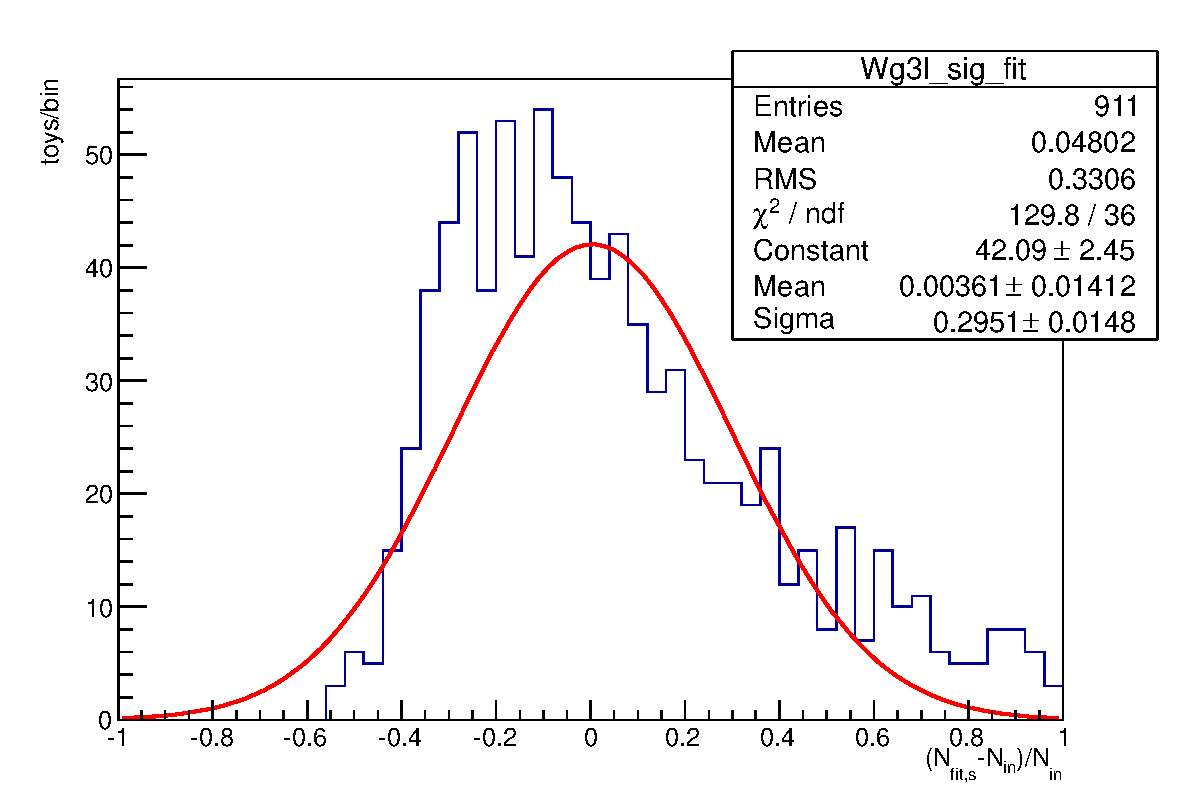
\includegraphics[width=.45\textwidth]{figures/norm_inj125_0j_125_sfit_Wg3l_xww.pdf}
} 

\caption{The relative fit bias $(N_{\text fit} - N_{\text in})/N_{\text in}$ distributions 
of the main signal and background processes in the toy MC based fit studies in the {\bf 0-Jet bin}. 
The toy datasets are generated sampling {\bf both statistics of the templates and systematic nusiances}. }
\label{fig:toyfit_0j}
\end{figure}
%%%%%%%%%%%%%%%%%%%%%%%%%%%%%%%%%%%%
